\documentclass{article}

\usepackage{pgf}
\usepackage{array}
\usepackage{caption}
\usepackage{booktabs}
\usepackage{multirow}
\usepackage{geometry}
\usepackage{subcaption}
\usepackage{pdflscape}
\usepackage{graphicx}
\usepackage[utf8]{inputenc}
\usepackage{pgfplots}

\pgfplotsset{compat=newest}
\usetikzlibrary{patterns,shapes.arrows}
\usepgfplotslibrary{groupplots,dateplot}
\geometry{paperwidth=32cm, paperheight=60cm, margin=1in}


\begin{document}
\pagestyle{empty}
\section{5-Fold Cross Validation}
\vspace{20pt}

\begin{table}[h!tbp]
  \centering
  \renewcommand{\arraystretch}{1.2}
  \begin{tabular}{lccc}
    \toprule
    \multirow{2}{*}{\textbf{Metrics}} & \multicolumn{3}{c}{\textbf{Scores}} \\
    \cmidrule(lr){2-4}
    & \textbf{Human}& \textbf{Mouse} & \textbf{Yeast} \\
    \midrule
    \textbf{Accuracy} & 0.80& 0.84 & 0.84 \\
    \textbf{Mathew's CC} & 0.60& 0.68 & 0.84 \\
    \textbf{Cohen's Kappa} & 0.60& 0.68 & 0.84 \\
    \textbf{Specificity} & 0.78& 0.78 & 0.84 \\
    \bottomrule
  \end{tabular}
  \caption{Classifier Metrics of all species}
\end{table}

\begin{table}[h!tbp]
    \centering
    \renewcommand{\arraystretch}{1.2}
    \begin{tabular}{r|cccc|cccc|cccc|}

      \multicolumn{1}{c}{}
      & \multicolumn{4}{c}{\textbf{Human}}
      & \multicolumn{4}{c}{\textbf{Mouse}}
      & \multicolumn{4}{c}{\textbf{Yeast}} \\

      \cline{2-13}
      & \textbf{Precision} & \textbf{Recall} & \textbf{F1-Score} & \textbf{Support} 
      & \textbf{Precision} & \textbf{Recall} & \textbf{F1-Score} & \textbf{Support}
      & \textbf{Precision} & \textbf{Recall} & \textbf{F1-Score} & \textbf{Support} \\
      \cline{2-13}
      \textbf{0} & 0.81 & 0.81 & 0.81 & 0.81
                 & 0.81 & 0.81 & 0.81 & 0.81
                 & 0.81 & 0.81 & 0.81 & 0.81 \\

      \textbf{1} & 0.79 & 0.79 & 0.79 & 0.79
                 & 0.79 & 0.79 & 0.79 & 0.79
                 & 0.79 & 0.79 & 0.79 & 0.79 \\
      \textbf{Macro Avg} & 0.80 & 0.80 & 0.80 & 0.80 
                         & 0.80 & 0.80 & 0.80 & 0.80 
                         & 0.80 & 0.80 & 0.80 & 0.80 \\
      \textbf{Weighted Avg} & 0.80 & 0.80 & 0.80 & 0.80
                            & 0.80 & 0.80 & 0.80 & 0.80
                            & 0.80 & 0.80 & 0.80 & 0.80 \\
      \cline{2-13}
    \end{tabular}
    \caption{Classifier Reports of all species}
  \end{table}


\begin{table}[h!tbp]
    \centering
    \begin{tabular}{ccc}
      % This file was created with tikzplotlib v0.10.1.
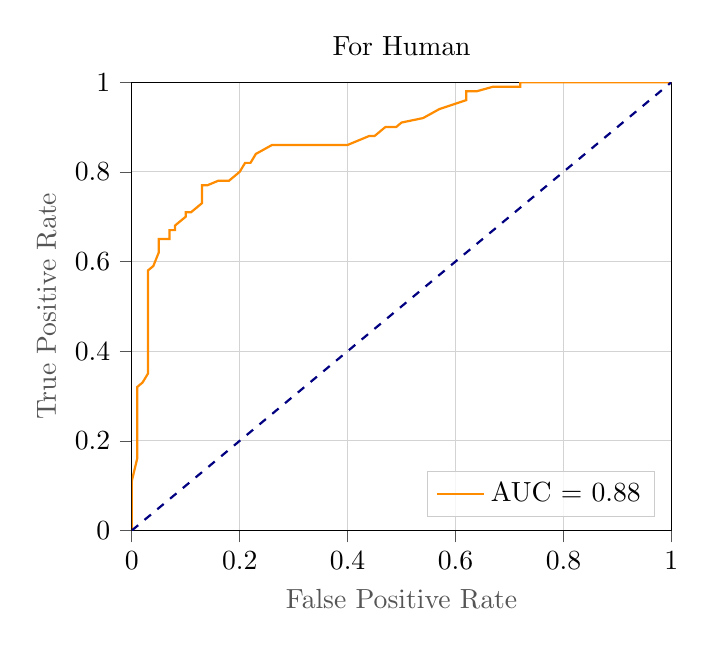
\begin{tikzpicture}

\definecolor{darkorange}{RGB}{255,140,0}
\definecolor{dimgray85}{RGB}{85,85,85}
\definecolor{lightgray}{RGB}{211,211,211}
\definecolor{lightgray204}{RGB}{204,204,204}
\definecolor{navy}{RGB}{0,0,128}

\begin{axis}[
legend cell align={left},
legend style={
  fill opacity=0.8,
  draw opacity=1,
  text opacity=1,
  at={(0.97,0.03)},
  anchor=south east,
  draw=lightgray204
},
tick align=outside,
tick pos=left,
title={For Human},
x grid style={lightgray},
xlabel=\textcolor{dimgray85}{False Positive Rate},
xmajorgrids,
xmin=0, xmax=1,
xtick style={color=dimgray85},
y grid style={lightgray},
ylabel=\textcolor{dimgray85}{True Positive Rate},
ymajorgrids,
ymin=0, ymax=1,
ytick style={color=dimgray85}
]
\addplot [thick, darkorange]
table {%
0 0
0 0.02
0 0.05
0 0.07
0 0.11
0.01 0.16
0.01 0.2
0.01 0.32
0.02 0.33
0.03 0.35
0.03 0.36
0.03 0.4
0.03 0.42
0.03 0.5
0.03 0.51
0.03 0.54
0.03 0.58
0.04 0.59
0.05 0.62
0.05 0.65
0.07 0.65
0.07 0.67
0.08 0.67
0.08 0.68
0.1 0.7
0.1 0.71
0.11 0.71
0.13 0.73
0.13 0.77
0.14 0.77
0.16 0.78
0.18 0.78
0.2 0.8
0.21 0.82
0.22 0.82
0.23 0.84
0.26 0.86
0.27 0.86
0.31 0.86
0.32 0.86
0.34 0.86
0.4 0.86
0.44 0.88
0.45 0.88
0.47 0.9
0.49 0.9
0.5 0.91
0.54 0.92
0.57 0.94
0.62 0.96
0.62 0.98
0.64 0.98
0.67 0.99
0.72 0.99
0.72 1
0.73 1
0.76 1
0.78 1
0.79 1
0.83 1
0.85 1
0.87 1
0.9 1
0.93 1
0.97 1
1 1
};
\addlegendentry{AUC = 0.88}
\addplot [thick, navy, dashed, forget plot]
table {%
0 0
1 1
};
\end{axis}

\end{tikzpicture}
&% This file was created with tikzplotlib v0.10.1.
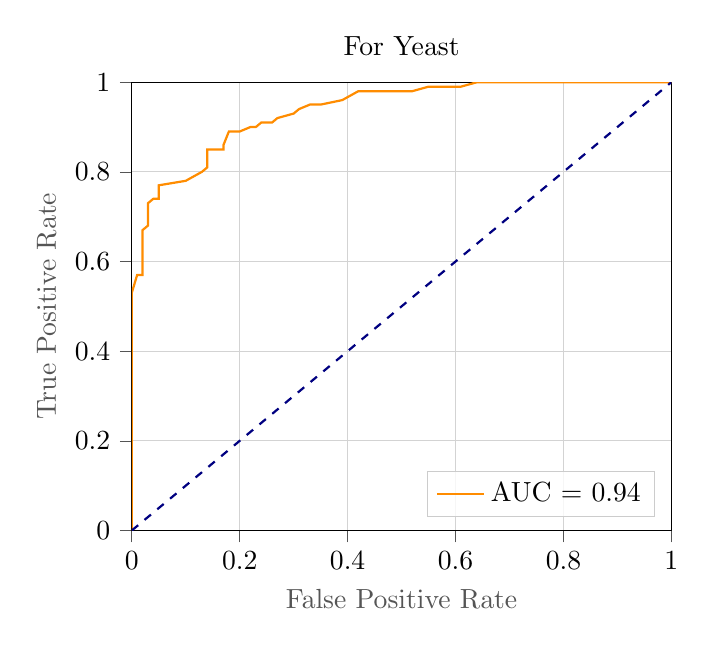
\begin{tikzpicture}

\definecolor{darkorange}{RGB}{255,140,0}
\definecolor{dimgray85}{RGB}{85,85,85}
\definecolor{lightgray}{RGB}{211,211,211}
\definecolor{lightgray204}{RGB}{204,204,204}
\definecolor{navy}{RGB}{0,0,128}

\begin{axis}[
legend cell align={left},
legend style={
  fill opacity=0.8,
  draw opacity=1,
  text opacity=1,
  at={(0.97,0.03)},
  anchor=south east,
  draw=lightgray204
},
tick align=outside,
tick pos=left,
title={For Yeast},
x grid style={lightgray},
xlabel=\textcolor{dimgray85}{False Positive Rate},
xmajorgrids,
xmin=0, xmax=1,
xtick style={color=dimgray85},
y grid style={lightgray},
ylabel=\textcolor{dimgray85}{True Positive Rate},
ymajorgrids,
ymin=0, ymax=1,
ytick style={color=dimgray85}
]
\addplot [thick, darkorange]
table {%
0 0
0 0.04
0 0.05
0 0.09
0 0.1
0 0.12
0 0.16
0 0.19
0 0.25
0 0.26
0 0.29
0 0.33
0 0.36
0 0.38
0 0.42
0 0.44
0 0.5
0 0.52
0 0.53
0.01 0.57
0.02 0.57
0.02 0.67
0.03 0.68
0.03 0.69
0.03 0.73
0.04 0.74
0.05 0.74
0.05 0.76
0.05 0.77
0.1 0.78
0.13 0.8
0.14 0.81
0.14 0.85
0.17 0.85
0.17 0.86
0.18 0.89
0.2 0.89
0.22 0.9
0.23 0.9
0.24 0.91
0.26 0.91
0.27 0.92
0.3 0.93
0.31 0.94
0.33 0.95
0.35 0.95
0.39 0.96
0.42 0.98
0.46 0.98
0.49 0.98
0.51 0.98
0.52 0.98
0.55 0.99
0.57 0.99
0.61 0.99
0.64 1
0.66 1
0.69 1
0.7 1
0.72 1
0.73 1
0.75 1
0.77 1
0.8 1
0.88 1
0.89 1
0.92 1
0.95 1
0.97 1
1 1
};
\addlegendentry{AUC = 0.94}
\addplot [thick, navy, dashed, forget plot]
table {%
0 0
1 1
};
\end{axis}

\end{tikzpicture}
&% This file was created with tikzplotlib v0.10.1.
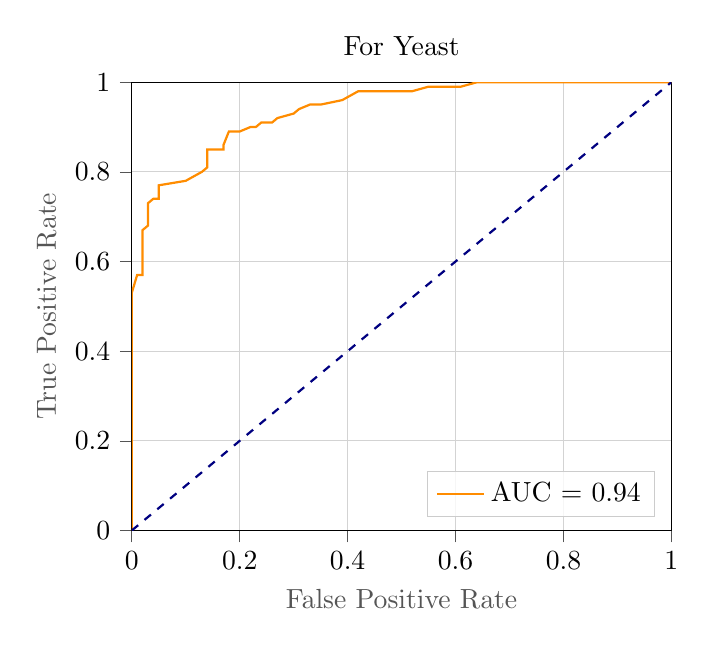
\begin{tikzpicture}

\definecolor{darkorange}{RGB}{255,140,0}
\definecolor{dimgray85}{RGB}{85,85,85}
\definecolor{lightgray}{RGB}{211,211,211}
\definecolor{lightgray204}{RGB}{204,204,204}
\definecolor{navy}{RGB}{0,0,128}

\begin{axis}[
legend cell align={left},
legend style={
  fill opacity=0.8,
  draw opacity=1,
  text opacity=1,
  at={(0.97,0.03)},
  anchor=south east,
  draw=lightgray204
},
tick align=outside,
tick pos=left,
title={For Yeast},
x grid style={lightgray},
xlabel=\textcolor{dimgray85}{False Positive Rate},
xmajorgrids,
xmin=0, xmax=1,
xtick style={color=dimgray85},
y grid style={lightgray},
ylabel=\textcolor{dimgray85}{True Positive Rate},
ymajorgrids,
ymin=0, ymax=1,
ytick style={color=dimgray85}
]
\addplot [thick, darkorange]
table {%
0 0
0 0.04
0 0.05
0 0.09
0 0.1
0 0.12
0 0.16
0 0.19
0 0.25
0 0.26
0 0.29
0 0.33
0 0.36
0 0.38
0 0.42
0 0.44
0 0.5
0 0.52
0 0.53
0.01 0.57
0.02 0.57
0.02 0.67
0.03 0.68
0.03 0.69
0.03 0.73
0.04 0.74
0.05 0.74
0.05 0.76
0.05 0.77
0.1 0.78
0.13 0.8
0.14 0.81
0.14 0.85
0.17 0.85
0.17 0.86
0.18 0.89
0.2 0.89
0.22 0.9
0.23 0.9
0.24 0.91
0.26 0.91
0.27 0.92
0.3 0.93
0.31 0.94
0.33 0.95
0.35 0.95
0.39 0.96
0.42 0.98
0.46 0.98
0.49 0.98
0.51 0.98
0.52 0.98
0.55 0.99
0.57 0.99
0.61 0.99
0.64 1
0.66 1
0.69 1
0.7 1
0.72 1
0.73 1
0.75 1
0.77 1
0.8 1
0.88 1
0.89 1
0.92 1
0.95 1
0.97 1
1 1
};
\addlegendentry{AUC = 0.94}
\addplot [thick, navy, dashed, forget plot]
table {%
0 0
1 1
};
\end{axis}

\end{tikzpicture}
 \\
    \end{tabular}
    \caption{Receiver operating characteristic (ROC) curves}
\end{table}

\begin{table}[h!tbp]
    \centering
    \begin{tabular}{ccc}
      % This file was created with tikzplotlib v0.10.1.
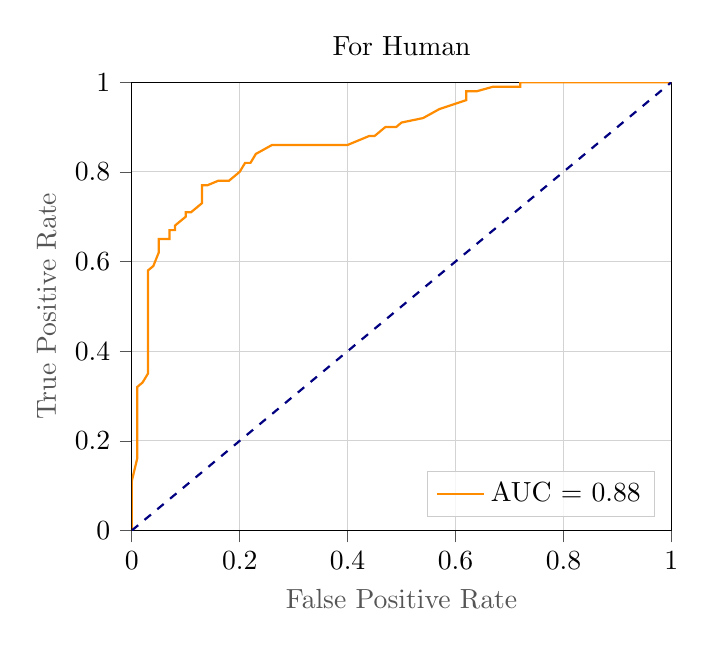
\begin{tikzpicture}

\definecolor{darkorange}{RGB}{255,140,0}
\definecolor{dimgray85}{RGB}{85,85,85}
\definecolor{lightgray}{RGB}{211,211,211}
\definecolor{lightgray204}{RGB}{204,204,204}
\definecolor{navy}{RGB}{0,0,128}

\begin{axis}[
legend cell align={left},
legend style={
  fill opacity=0.8,
  draw opacity=1,
  text opacity=1,
  at={(0.97,0.03)},
  anchor=south east,
  draw=lightgray204
},
tick align=outside,
tick pos=left,
title={For Human},
x grid style={lightgray},
xlabel=\textcolor{dimgray85}{False Positive Rate},
xmajorgrids,
xmin=0, xmax=1,
xtick style={color=dimgray85},
y grid style={lightgray},
ylabel=\textcolor{dimgray85}{True Positive Rate},
ymajorgrids,
ymin=0, ymax=1,
ytick style={color=dimgray85}
]
\addplot [thick, darkorange]
table {%
0 0
0 0.02
0 0.05
0 0.07
0 0.11
0.01 0.16
0.01 0.2
0.01 0.32
0.02 0.33
0.03 0.35
0.03 0.36
0.03 0.4
0.03 0.42
0.03 0.5
0.03 0.51
0.03 0.54
0.03 0.58
0.04 0.59
0.05 0.62
0.05 0.65
0.07 0.65
0.07 0.67
0.08 0.67
0.08 0.68
0.1 0.7
0.1 0.71
0.11 0.71
0.13 0.73
0.13 0.77
0.14 0.77
0.16 0.78
0.18 0.78
0.2 0.8
0.21 0.82
0.22 0.82
0.23 0.84
0.26 0.86
0.27 0.86
0.31 0.86
0.32 0.86
0.34 0.86
0.4 0.86
0.44 0.88
0.45 0.88
0.47 0.9
0.49 0.9
0.5 0.91
0.54 0.92
0.57 0.94
0.62 0.96
0.62 0.98
0.64 0.98
0.67 0.99
0.72 0.99
0.72 1
0.73 1
0.76 1
0.78 1
0.79 1
0.83 1
0.85 1
0.87 1
0.9 1
0.93 1
0.97 1
1 1
};
\addlegendentry{AUC = 0.88}
\addplot [thick, navy, dashed, forget plot]
table {%
0 0
1 1
};
\end{axis}

\end{tikzpicture}
&% This file was created with tikzplotlib v0.10.1.
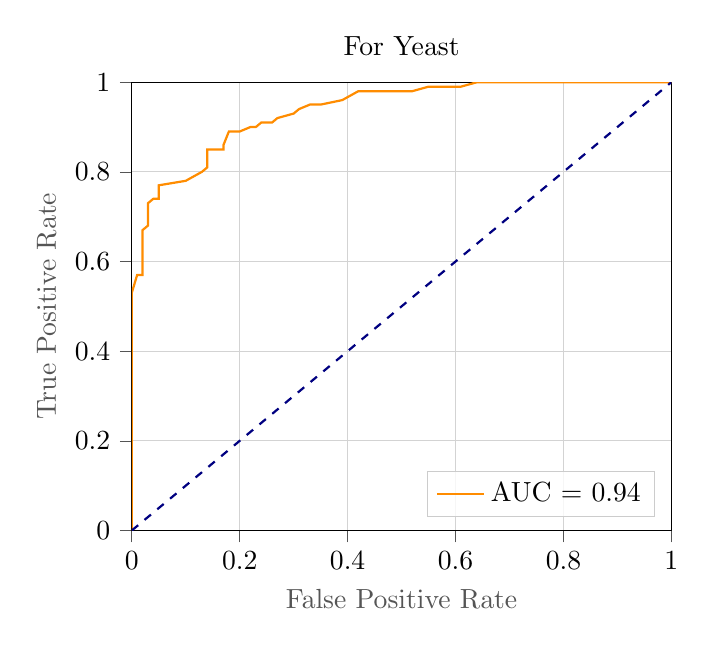
\begin{tikzpicture}

\definecolor{darkorange}{RGB}{255,140,0}
\definecolor{dimgray85}{RGB}{85,85,85}
\definecolor{lightgray}{RGB}{211,211,211}
\definecolor{lightgray204}{RGB}{204,204,204}
\definecolor{navy}{RGB}{0,0,128}

\begin{axis}[
legend cell align={left},
legend style={
  fill opacity=0.8,
  draw opacity=1,
  text opacity=1,
  at={(0.97,0.03)},
  anchor=south east,
  draw=lightgray204
},
tick align=outside,
tick pos=left,
title={For Yeast},
x grid style={lightgray},
xlabel=\textcolor{dimgray85}{False Positive Rate},
xmajorgrids,
xmin=0, xmax=1,
xtick style={color=dimgray85},
y grid style={lightgray},
ylabel=\textcolor{dimgray85}{True Positive Rate},
ymajorgrids,
ymin=0, ymax=1,
ytick style={color=dimgray85}
]
\addplot [thick, darkorange]
table {%
0 0
0 0.04
0 0.05
0 0.09
0 0.1
0 0.12
0 0.16
0 0.19
0 0.25
0 0.26
0 0.29
0 0.33
0 0.36
0 0.38
0 0.42
0 0.44
0 0.5
0 0.52
0 0.53
0.01 0.57
0.02 0.57
0.02 0.67
0.03 0.68
0.03 0.69
0.03 0.73
0.04 0.74
0.05 0.74
0.05 0.76
0.05 0.77
0.1 0.78
0.13 0.8
0.14 0.81
0.14 0.85
0.17 0.85
0.17 0.86
0.18 0.89
0.2 0.89
0.22 0.9
0.23 0.9
0.24 0.91
0.26 0.91
0.27 0.92
0.3 0.93
0.31 0.94
0.33 0.95
0.35 0.95
0.39 0.96
0.42 0.98
0.46 0.98
0.49 0.98
0.51 0.98
0.52 0.98
0.55 0.99
0.57 0.99
0.61 0.99
0.64 1
0.66 1
0.69 1
0.7 1
0.72 1
0.73 1
0.75 1
0.77 1
0.8 1
0.88 1
0.89 1
0.92 1
0.95 1
0.97 1
1 1
};
\addlegendentry{AUC = 0.94}
\addplot [thick, navy, dashed, forget plot]
table {%
0 0
1 1
};
\end{axis}

\end{tikzpicture}
&% This file was created with tikzplotlib v0.10.1.
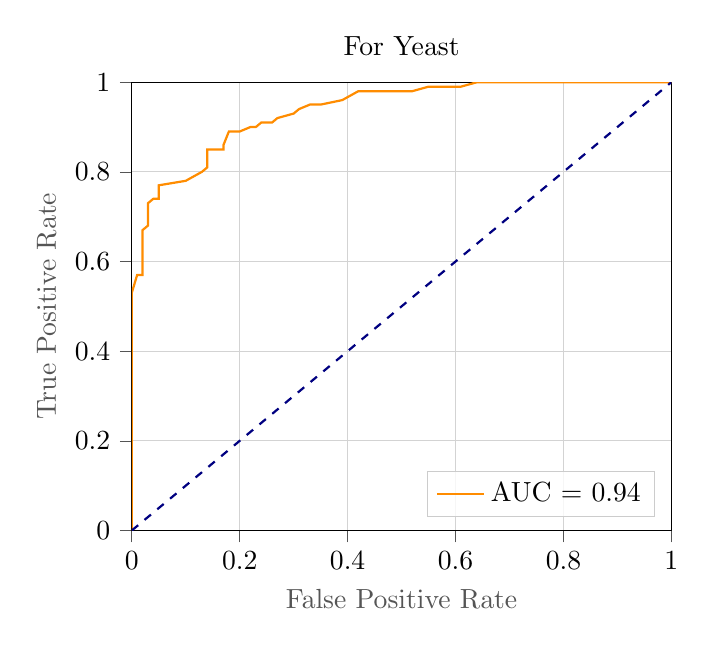
\begin{tikzpicture}

\definecolor{darkorange}{RGB}{255,140,0}
\definecolor{dimgray85}{RGB}{85,85,85}
\definecolor{lightgray}{RGB}{211,211,211}
\definecolor{lightgray204}{RGB}{204,204,204}
\definecolor{navy}{RGB}{0,0,128}

\begin{axis}[
legend cell align={left},
legend style={
  fill opacity=0.8,
  draw opacity=1,
  text opacity=1,
  at={(0.97,0.03)},
  anchor=south east,
  draw=lightgray204
},
tick align=outside,
tick pos=left,
title={For Yeast},
x grid style={lightgray},
xlabel=\textcolor{dimgray85}{False Positive Rate},
xmajorgrids,
xmin=0, xmax=1,
xtick style={color=dimgray85},
y grid style={lightgray},
ylabel=\textcolor{dimgray85}{True Positive Rate},
ymajorgrids,
ymin=0, ymax=1,
ytick style={color=dimgray85}
]
\addplot [thick, darkorange]
table {%
0 0
0 0.04
0 0.05
0 0.09
0 0.1
0 0.12
0 0.16
0 0.19
0 0.25
0 0.26
0 0.29
0 0.33
0 0.36
0 0.38
0 0.42
0 0.44
0 0.5
0 0.52
0 0.53
0.01 0.57
0.02 0.57
0.02 0.67
0.03 0.68
0.03 0.69
0.03 0.73
0.04 0.74
0.05 0.74
0.05 0.76
0.05 0.77
0.1 0.78
0.13 0.8
0.14 0.81
0.14 0.85
0.17 0.85
0.17 0.86
0.18 0.89
0.2 0.89
0.22 0.9
0.23 0.9
0.24 0.91
0.26 0.91
0.27 0.92
0.3 0.93
0.31 0.94
0.33 0.95
0.35 0.95
0.39 0.96
0.42 0.98
0.46 0.98
0.49 0.98
0.51 0.98
0.52 0.98
0.55 0.99
0.57 0.99
0.61 0.99
0.64 1
0.66 1
0.69 1
0.7 1
0.72 1
0.73 1
0.75 1
0.77 1
0.8 1
0.88 1
0.89 1
0.92 1
0.95 1
0.97 1
1 1
};
\addlegendentry{AUC = 0.94}
\addplot [thick, navy, dashed, forget plot]
table {%
0 0
1 1
};
\end{axis}

\end{tikzpicture}
 \\
    \end{tabular}
    \caption{Receiver operating characteristic (ROC) curves}
\end{table}

\begin{table}[h!tbp]
    \centering
    \begin{tabular}{ccc}
      % This file was created with tikzplotlib v0.10.1.
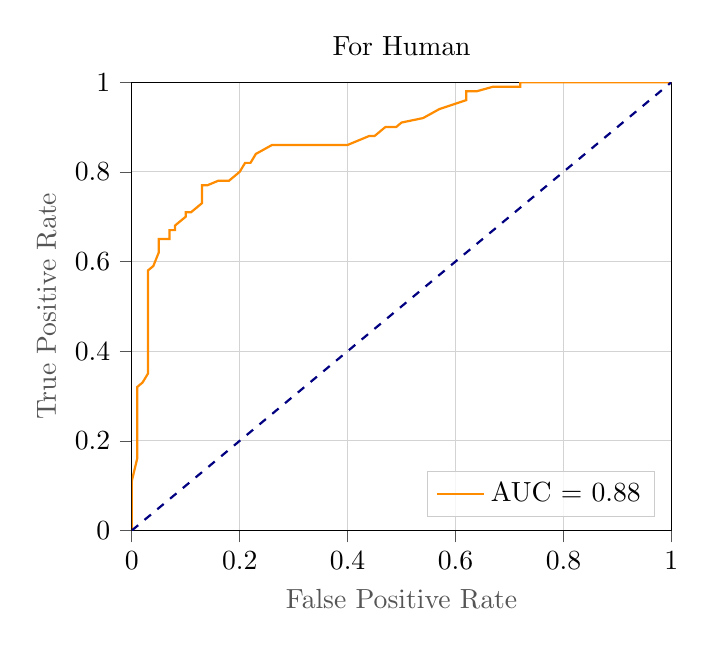
\begin{tikzpicture}

\definecolor{darkorange}{RGB}{255,140,0}
\definecolor{dimgray85}{RGB}{85,85,85}
\definecolor{lightgray}{RGB}{211,211,211}
\definecolor{lightgray204}{RGB}{204,204,204}
\definecolor{navy}{RGB}{0,0,128}

\begin{axis}[
legend cell align={left},
legend style={
  fill opacity=0.8,
  draw opacity=1,
  text opacity=1,
  at={(0.97,0.03)},
  anchor=south east,
  draw=lightgray204
},
tick align=outside,
tick pos=left,
title={For Human},
x grid style={lightgray},
xlabel=\textcolor{dimgray85}{False Positive Rate},
xmajorgrids,
xmin=0, xmax=1,
xtick style={color=dimgray85},
y grid style={lightgray},
ylabel=\textcolor{dimgray85}{True Positive Rate},
ymajorgrids,
ymin=0, ymax=1,
ytick style={color=dimgray85}
]
\addplot [thick, darkorange]
table {%
0 0
0 0.02
0 0.05
0 0.07
0 0.11
0.01 0.16
0.01 0.2
0.01 0.32
0.02 0.33
0.03 0.35
0.03 0.36
0.03 0.4
0.03 0.42
0.03 0.5
0.03 0.51
0.03 0.54
0.03 0.58
0.04 0.59
0.05 0.62
0.05 0.65
0.07 0.65
0.07 0.67
0.08 0.67
0.08 0.68
0.1 0.7
0.1 0.71
0.11 0.71
0.13 0.73
0.13 0.77
0.14 0.77
0.16 0.78
0.18 0.78
0.2 0.8
0.21 0.82
0.22 0.82
0.23 0.84
0.26 0.86
0.27 0.86
0.31 0.86
0.32 0.86
0.34 0.86
0.4 0.86
0.44 0.88
0.45 0.88
0.47 0.9
0.49 0.9
0.5 0.91
0.54 0.92
0.57 0.94
0.62 0.96
0.62 0.98
0.64 0.98
0.67 0.99
0.72 0.99
0.72 1
0.73 1
0.76 1
0.78 1
0.79 1
0.83 1
0.85 1
0.87 1
0.9 1
0.93 1
0.97 1
1 1
};
\addlegendentry{AUC = 0.88}
\addplot [thick, navy, dashed, forget plot]
table {%
0 0
1 1
};
\end{axis}

\end{tikzpicture}
&% This file was created with tikzplotlib v0.10.1.
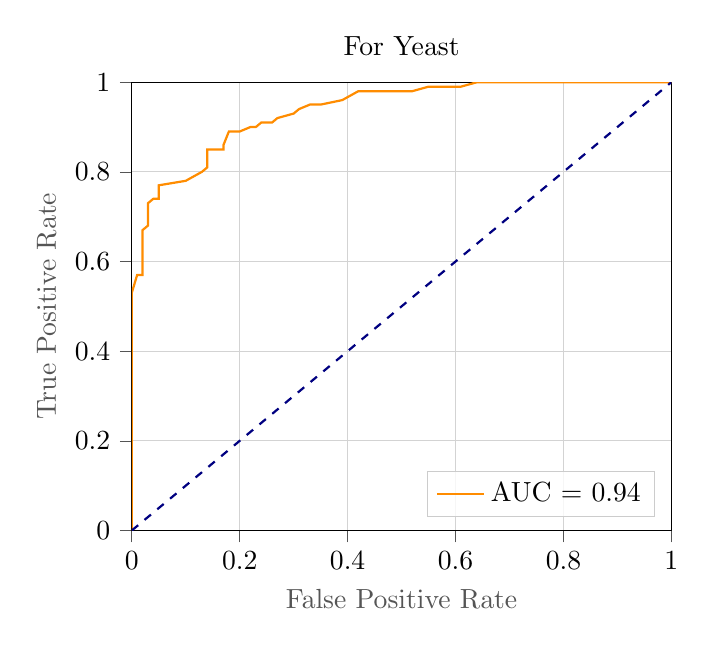
\begin{tikzpicture}

\definecolor{darkorange}{RGB}{255,140,0}
\definecolor{dimgray85}{RGB}{85,85,85}
\definecolor{lightgray}{RGB}{211,211,211}
\definecolor{lightgray204}{RGB}{204,204,204}
\definecolor{navy}{RGB}{0,0,128}

\begin{axis}[
legend cell align={left},
legend style={
  fill opacity=0.8,
  draw opacity=1,
  text opacity=1,
  at={(0.97,0.03)},
  anchor=south east,
  draw=lightgray204
},
tick align=outside,
tick pos=left,
title={For Yeast},
x grid style={lightgray},
xlabel=\textcolor{dimgray85}{False Positive Rate},
xmajorgrids,
xmin=0, xmax=1,
xtick style={color=dimgray85},
y grid style={lightgray},
ylabel=\textcolor{dimgray85}{True Positive Rate},
ymajorgrids,
ymin=0, ymax=1,
ytick style={color=dimgray85}
]
\addplot [thick, darkorange]
table {%
0 0
0 0.04
0 0.05
0 0.09
0 0.1
0 0.12
0 0.16
0 0.19
0 0.25
0 0.26
0 0.29
0 0.33
0 0.36
0 0.38
0 0.42
0 0.44
0 0.5
0 0.52
0 0.53
0.01 0.57
0.02 0.57
0.02 0.67
0.03 0.68
0.03 0.69
0.03 0.73
0.04 0.74
0.05 0.74
0.05 0.76
0.05 0.77
0.1 0.78
0.13 0.8
0.14 0.81
0.14 0.85
0.17 0.85
0.17 0.86
0.18 0.89
0.2 0.89
0.22 0.9
0.23 0.9
0.24 0.91
0.26 0.91
0.27 0.92
0.3 0.93
0.31 0.94
0.33 0.95
0.35 0.95
0.39 0.96
0.42 0.98
0.46 0.98
0.49 0.98
0.51 0.98
0.52 0.98
0.55 0.99
0.57 0.99
0.61 0.99
0.64 1
0.66 1
0.69 1
0.7 1
0.72 1
0.73 1
0.75 1
0.77 1
0.8 1
0.88 1
0.89 1
0.92 1
0.95 1
0.97 1
1 1
};
\addlegendentry{AUC = 0.94}
\addplot [thick, navy, dashed, forget plot]
table {%
0 0
1 1
};
\end{axis}

\end{tikzpicture}
&% This file was created with tikzplotlib v0.10.1.
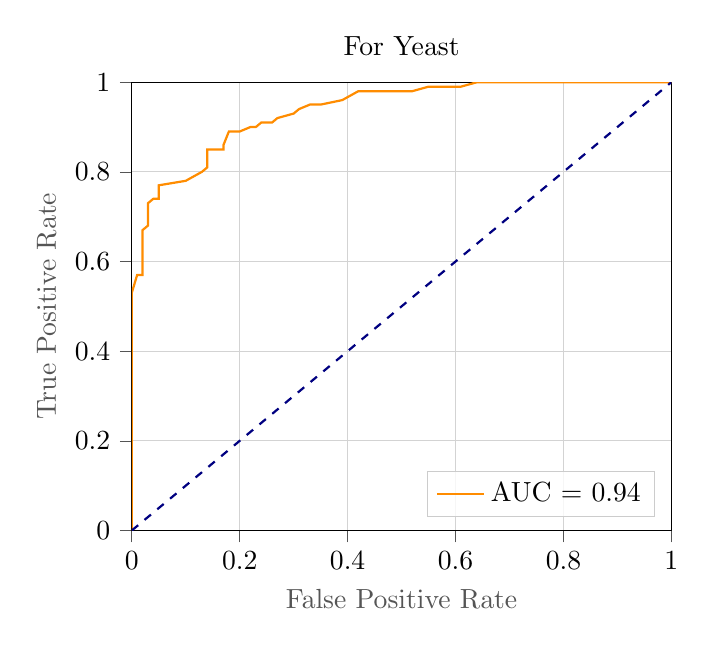
\begin{tikzpicture}

\definecolor{darkorange}{RGB}{255,140,0}
\definecolor{dimgray85}{RGB}{85,85,85}
\definecolor{lightgray}{RGB}{211,211,211}
\definecolor{lightgray204}{RGB}{204,204,204}
\definecolor{navy}{RGB}{0,0,128}

\begin{axis}[
legend cell align={left},
legend style={
  fill opacity=0.8,
  draw opacity=1,
  text opacity=1,
  at={(0.97,0.03)},
  anchor=south east,
  draw=lightgray204
},
tick align=outside,
tick pos=left,
title={For Yeast},
x grid style={lightgray},
xlabel=\textcolor{dimgray85}{False Positive Rate},
xmajorgrids,
xmin=0, xmax=1,
xtick style={color=dimgray85},
y grid style={lightgray},
ylabel=\textcolor{dimgray85}{True Positive Rate},
ymajorgrids,
ymin=0, ymax=1,
ytick style={color=dimgray85}
]
\addplot [thick, darkorange]
table {%
0 0
0 0.04
0 0.05
0 0.09
0 0.1
0 0.12
0 0.16
0 0.19
0 0.25
0 0.26
0 0.29
0 0.33
0 0.36
0 0.38
0 0.42
0 0.44
0 0.5
0 0.52
0 0.53
0.01 0.57
0.02 0.57
0.02 0.67
0.03 0.68
0.03 0.69
0.03 0.73
0.04 0.74
0.05 0.74
0.05 0.76
0.05 0.77
0.1 0.78
0.13 0.8
0.14 0.81
0.14 0.85
0.17 0.85
0.17 0.86
0.18 0.89
0.2 0.89
0.22 0.9
0.23 0.9
0.24 0.91
0.26 0.91
0.27 0.92
0.3 0.93
0.31 0.94
0.33 0.95
0.35 0.95
0.39 0.96
0.42 0.98
0.46 0.98
0.49 0.98
0.51 0.98
0.52 0.98
0.55 0.99
0.57 0.99
0.61 0.99
0.64 1
0.66 1
0.69 1
0.7 1
0.72 1
0.73 1
0.75 1
0.77 1
0.8 1
0.88 1
0.89 1
0.92 1
0.95 1
0.97 1
1 1
};
\addlegendentry{AUC = 0.94}
\addplot [thick, navy, dashed, forget plot]
table {%
0 0
1 1
};
\end{axis}

\end{tikzpicture}
 \\
    \end{tabular}
    \caption{Receiver operating characteristic (ROC) curves}
\end{table}

\begin{table}[h!tbp]
    \centering
    \begin{tabular}{ccc}
      % This file was created with tikzplotlib v0.10.1.
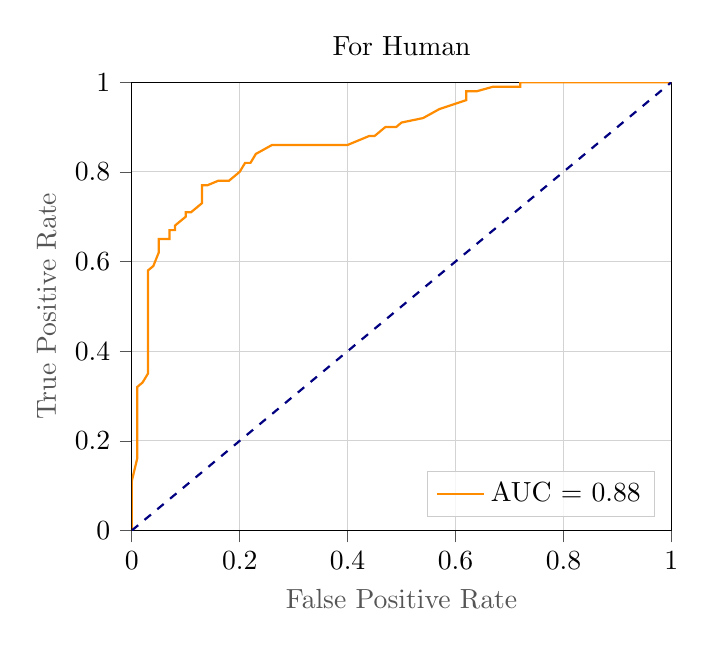
\begin{tikzpicture}

\definecolor{darkorange}{RGB}{255,140,0}
\definecolor{dimgray85}{RGB}{85,85,85}
\definecolor{lightgray}{RGB}{211,211,211}
\definecolor{lightgray204}{RGB}{204,204,204}
\definecolor{navy}{RGB}{0,0,128}

\begin{axis}[
legend cell align={left},
legend style={
  fill opacity=0.8,
  draw opacity=1,
  text opacity=1,
  at={(0.97,0.03)},
  anchor=south east,
  draw=lightgray204
},
tick align=outside,
tick pos=left,
title={For Human},
x grid style={lightgray},
xlabel=\textcolor{dimgray85}{False Positive Rate},
xmajorgrids,
xmin=0, xmax=1,
xtick style={color=dimgray85},
y grid style={lightgray},
ylabel=\textcolor{dimgray85}{True Positive Rate},
ymajorgrids,
ymin=0, ymax=1,
ytick style={color=dimgray85}
]
\addplot [thick, darkorange]
table {%
0 0
0 0.02
0 0.05
0 0.07
0 0.11
0.01 0.16
0.01 0.2
0.01 0.32
0.02 0.33
0.03 0.35
0.03 0.36
0.03 0.4
0.03 0.42
0.03 0.5
0.03 0.51
0.03 0.54
0.03 0.58
0.04 0.59
0.05 0.62
0.05 0.65
0.07 0.65
0.07 0.67
0.08 0.67
0.08 0.68
0.1 0.7
0.1 0.71
0.11 0.71
0.13 0.73
0.13 0.77
0.14 0.77
0.16 0.78
0.18 0.78
0.2 0.8
0.21 0.82
0.22 0.82
0.23 0.84
0.26 0.86
0.27 0.86
0.31 0.86
0.32 0.86
0.34 0.86
0.4 0.86
0.44 0.88
0.45 0.88
0.47 0.9
0.49 0.9
0.5 0.91
0.54 0.92
0.57 0.94
0.62 0.96
0.62 0.98
0.64 0.98
0.67 0.99
0.72 0.99
0.72 1
0.73 1
0.76 1
0.78 1
0.79 1
0.83 1
0.85 1
0.87 1
0.9 1
0.93 1
0.97 1
1 1
};
\addlegendentry{AUC = 0.88}
\addplot [thick, navy, dashed, forget plot]
table {%
0 0
1 1
};
\end{axis}

\end{tikzpicture}
&% This file was created with tikzplotlib v0.10.1.
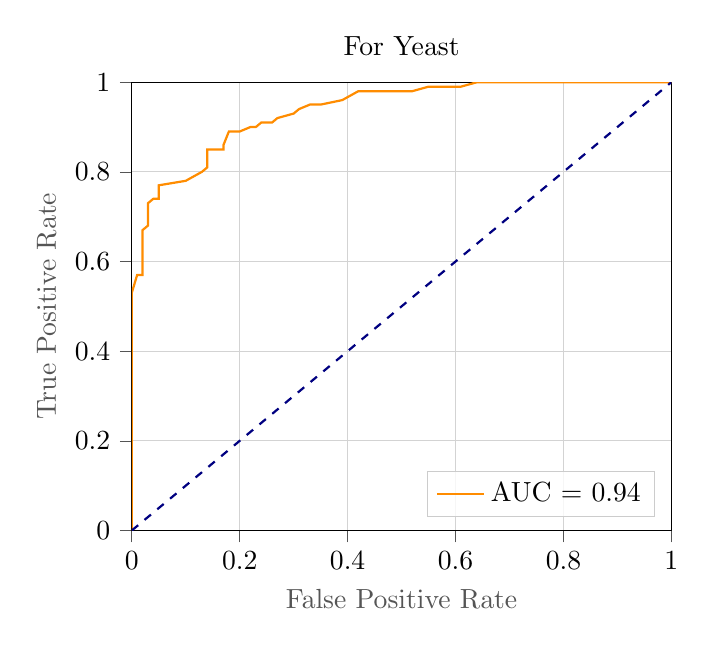
\begin{tikzpicture}

\definecolor{darkorange}{RGB}{255,140,0}
\definecolor{dimgray85}{RGB}{85,85,85}
\definecolor{lightgray}{RGB}{211,211,211}
\definecolor{lightgray204}{RGB}{204,204,204}
\definecolor{navy}{RGB}{0,0,128}

\begin{axis}[
legend cell align={left},
legend style={
  fill opacity=0.8,
  draw opacity=1,
  text opacity=1,
  at={(0.97,0.03)},
  anchor=south east,
  draw=lightgray204
},
tick align=outside,
tick pos=left,
title={For Yeast},
x grid style={lightgray},
xlabel=\textcolor{dimgray85}{False Positive Rate},
xmajorgrids,
xmin=0, xmax=1,
xtick style={color=dimgray85},
y grid style={lightgray},
ylabel=\textcolor{dimgray85}{True Positive Rate},
ymajorgrids,
ymin=0, ymax=1,
ytick style={color=dimgray85}
]
\addplot [thick, darkorange]
table {%
0 0
0 0.04
0 0.05
0 0.09
0 0.1
0 0.12
0 0.16
0 0.19
0 0.25
0 0.26
0 0.29
0 0.33
0 0.36
0 0.38
0 0.42
0 0.44
0 0.5
0 0.52
0 0.53
0.01 0.57
0.02 0.57
0.02 0.67
0.03 0.68
0.03 0.69
0.03 0.73
0.04 0.74
0.05 0.74
0.05 0.76
0.05 0.77
0.1 0.78
0.13 0.8
0.14 0.81
0.14 0.85
0.17 0.85
0.17 0.86
0.18 0.89
0.2 0.89
0.22 0.9
0.23 0.9
0.24 0.91
0.26 0.91
0.27 0.92
0.3 0.93
0.31 0.94
0.33 0.95
0.35 0.95
0.39 0.96
0.42 0.98
0.46 0.98
0.49 0.98
0.51 0.98
0.52 0.98
0.55 0.99
0.57 0.99
0.61 0.99
0.64 1
0.66 1
0.69 1
0.7 1
0.72 1
0.73 1
0.75 1
0.77 1
0.8 1
0.88 1
0.89 1
0.92 1
0.95 1
0.97 1
1 1
};
\addlegendentry{AUC = 0.94}
\addplot [thick, navy, dashed, forget plot]
table {%
0 0
1 1
};
\end{axis}

\end{tikzpicture}
&% This file was created with tikzplotlib v0.10.1.
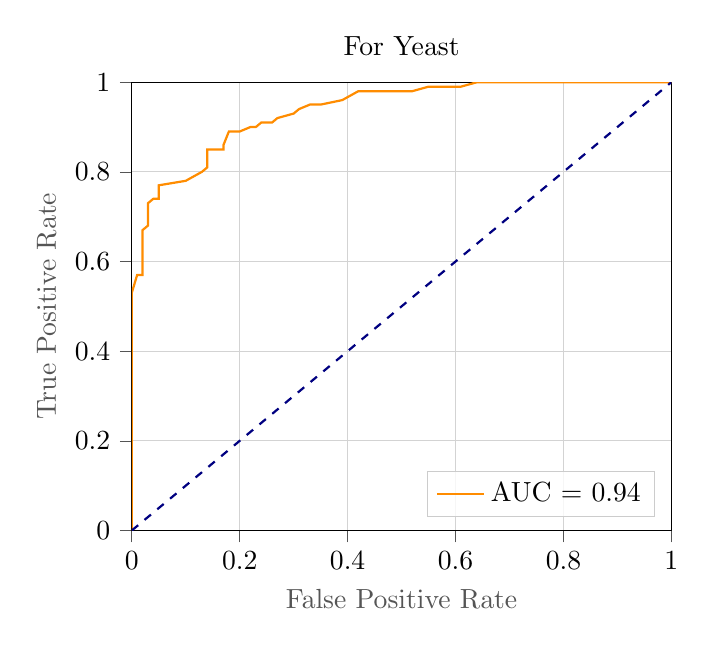
\begin{tikzpicture}

\definecolor{darkorange}{RGB}{255,140,0}
\definecolor{dimgray85}{RGB}{85,85,85}
\definecolor{lightgray}{RGB}{211,211,211}
\definecolor{lightgray204}{RGB}{204,204,204}
\definecolor{navy}{RGB}{0,0,128}

\begin{axis}[
legend cell align={left},
legend style={
  fill opacity=0.8,
  draw opacity=1,
  text opacity=1,
  at={(0.97,0.03)},
  anchor=south east,
  draw=lightgray204
},
tick align=outside,
tick pos=left,
title={For Yeast},
x grid style={lightgray},
xlabel=\textcolor{dimgray85}{False Positive Rate},
xmajorgrids,
xmin=0, xmax=1,
xtick style={color=dimgray85},
y grid style={lightgray},
ylabel=\textcolor{dimgray85}{True Positive Rate},
ymajorgrids,
ymin=0, ymax=1,
ytick style={color=dimgray85}
]
\addplot [thick, darkorange]
table {%
0 0
0 0.04
0 0.05
0 0.09
0 0.1
0 0.12
0 0.16
0 0.19
0 0.25
0 0.26
0 0.29
0 0.33
0 0.36
0 0.38
0 0.42
0 0.44
0 0.5
0 0.52
0 0.53
0.01 0.57
0.02 0.57
0.02 0.67
0.03 0.68
0.03 0.69
0.03 0.73
0.04 0.74
0.05 0.74
0.05 0.76
0.05 0.77
0.1 0.78
0.13 0.8
0.14 0.81
0.14 0.85
0.17 0.85
0.17 0.86
0.18 0.89
0.2 0.89
0.22 0.9
0.23 0.9
0.24 0.91
0.26 0.91
0.27 0.92
0.3 0.93
0.31 0.94
0.33 0.95
0.35 0.95
0.39 0.96
0.42 0.98
0.46 0.98
0.49 0.98
0.51 0.98
0.52 0.98
0.55 0.99
0.57 0.99
0.61 0.99
0.64 1
0.66 1
0.69 1
0.7 1
0.72 1
0.73 1
0.75 1
0.77 1
0.8 1
0.88 1
0.89 1
0.92 1
0.95 1
0.97 1
1 1
};
\addlegendentry{AUC = 0.94}
\addplot [thick, navy, dashed, forget plot]
table {%
0 0
1 1
};
\end{axis}

\end{tikzpicture}
 \\
    \end{tabular}
    \caption{Receiver operating characteristic (ROC) curves}
\end{table}

\end{document}
\begin{table}
  \begin{tabular}{ccc}
    % This file was created with tikzplotlib v0.10.1.
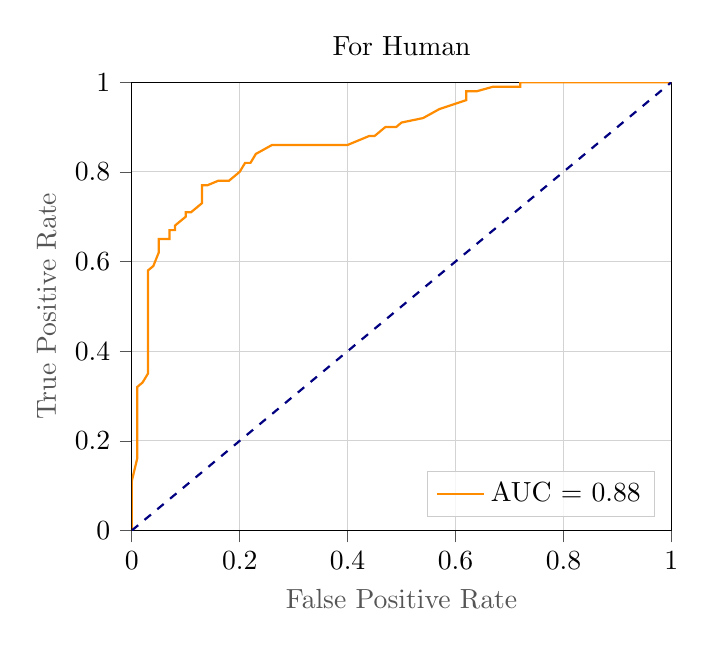
\begin{tikzpicture}

\definecolor{darkorange}{RGB}{255,140,0}
\definecolor{dimgray85}{RGB}{85,85,85}
\definecolor{lightgray}{RGB}{211,211,211}
\definecolor{lightgray204}{RGB}{204,204,204}
\definecolor{navy}{RGB}{0,0,128}

\begin{axis}[
legend cell align={left},
legend style={
  fill opacity=0.8,
  draw opacity=1,
  text opacity=1,
  at={(0.97,0.03)},
  anchor=south east,
  draw=lightgray204
},
tick align=outside,
tick pos=left,
title={For Human},
x grid style={lightgray},
xlabel=\textcolor{dimgray85}{False Positive Rate},
xmajorgrids,
xmin=0, xmax=1,
xtick style={color=dimgray85},
y grid style={lightgray},
ylabel=\textcolor{dimgray85}{True Positive Rate},
ymajorgrids,
ymin=0, ymax=1,
ytick style={color=dimgray85}
]
\addplot [thick, darkorange]
table {%
0 0
0 0.02
0 0.05
0 0.07
0 0.11
0.01 0.16
0.01 0.2
0.01 0.32
0.02 0.33
0.03 0.35
0.03 0.36
0.03 0.4
0.03 0.42
0.03 0.5
0.03 0.51
0.03 0.54
0.03 0.58
0.04 0.59
0.05 0.62
0.05 0.65
0.07 0.65
0.07 0.67
0.08 0.67
0.08 0.68
0.1 0.7
0.1 0.71
0.11 0.71
0.13 0.73
0.13 0.77
0.14 0.77
0.16 0.78
0.18 0.78
0.2 0.8
0.21 0.82
0.22 0.82
0.23 0.84
0.26 0.86
0.27 0.86
0.31 0.86
0.32 0.86
0.34 0.86
0.4 0.86
0.44 0.88
0.45 0.88
0.47 0.9
0.49 0.9
0.5 0.91
0.54 0.92
0.57 0.94
0.62 0.96
0.62 0.98
0.64 0.98
0.67 0.99
0.72 0.99
0.72 1
0.73 1
0.76 1
0.78 1
0.79 1
0.83 1
0.85 1
0.87 1
0.9 1
0.93 1
0.97 1
1 1
};
\addlegendentry{AUC = 0.88}
\addplot [thick, navy, dashed, forget plot]
table {%
0 0
1 1
};
\end{axis}

\end{tikzpicture}
&% This file was created with tikzplotlib v0.10.1.
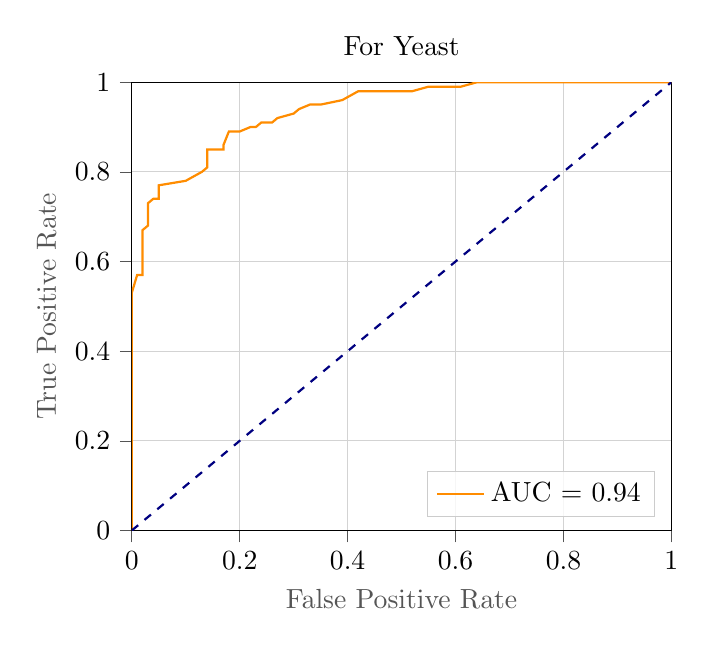
\begin{tikzpicture}

\definecolor{darkorange}{RGB}{255,140,0}
\definecolor{dimgray85}{RGB}{85,85,85}
\definecolor{lightgray}{RGB}{211,211,211}
\definecolor{lightgray204}{RGB}{204,204,204}
\definecolor{navy}{RGB}{0,0,128}

\begin{axis}[
legend cell align={left},
legend style={
  fill opacity=0.8,
  draw opacity=1,
  text opacity=1,
  at={(0.97,0.03)},
  anchor=south east,
  draw=lightgray204
},
tick align=outside,
tick pos=left,
title={For Yeast},
x grid style={lightgray},
xlabel=\textcolor{dimgray85}{False Positive Rate},
xmajorgrids,
xmin=0, xmax=1,
xtick style={color=dimgray85},
y grid style={lightgray},
ylabel=\textcolor{dimgray85}{True Positive Rate},
ymajorgrids,
ymin=0, ymax=1,
ytick style={color=dimgray85}
]
\addplot [thick, darkorange]
table {%
0 0
0 0.04
0 0.05
0 0.09
0 0.1
0 0.12
0 0.16
0 0.19
0 0.25
0 0.26
0 0.29
0 0.33
0 0.36
0 0.38
0 0.42
0 0.44
0 0.5
0 0.52
0 0.53
0.01 0.57
0.02 0.57
0.02 0.67
0.03 0.68
0.03 0.69
0.03 0.73
0.04 0.74
0.05 0.74
0.05 0.76
0.05 0.77
0.1 0.78
0.13 0.8
0.14 0.81
0.14 0.85
0.17 0.85
0.17 0.86
0.18 0.89
0.2 0.89
0.22 0.9
0.23 0.9
0.24 0.91
0.26 0.91
0.27 0.92
0.3 0.93
0.31 0.94
0.33 0.95
0.35 0.95
0.39 0.96
0.42 0.98
0.46 0.98
0.49 0.98
0.51 0.98
0.52 0.98
0.55 0.99
0.57 0.99
0.61 0.99
0.64 1
0.66 1
0.69 1
0.7 1
0.72 1
0.73 1
0.75 1
0.77 1
0.8 1
0.88 1
0.89 1
0.92 1
0.95 1
0.97 1
1 1
};
\addlegendentry{AUC = 0.94}
\addplot [thick, navy, dashed, forget plot]
table {%
0 0
1 1
};
\end{axis}

\end{tikzpicture}
 \\
  \end{tabular}
  \caption{Receiver operating characteristic (ROC) curves}
\end{table}
